\chapter{Theory of neutrino physics}\label{sec:NeutrinoTheory}

Just give a short overview of the historical context, but mainly focusing on the actual description of the neutrino theory, mostly stating the fact rather than giving a large background
1.neutrino interactions (neutrinos in the SM) - detection of neutrinos?
2.neutrino oscillations (including possible sterile oscillation) - maybe current status?
3.neutrino masses (theoretical prediction for their origins and their measurements)

I should discuss everything that is even briefly mentioned in the neutrino magnetic moment theory section.
\begin{itemize}
\item Dirac vs Majorana neutrinos
\item Neutrino masses
\item Neutrino interactions with electrons and nuclei
\item Neutrino oscillations and their implications
\end{itemize}

The story:
\begin{enumerate}
\item Brief history up to neutrinos being in the SM
\item Description of neutrinos in the SM
\item Interactions of neutrinos and their detection
\item Production of neutrinos
\item Solar and atmospheric neutrino anomalies and neutrino oscillations
\item Detail of neutrino oscillations for three flavours
\item Current state of neutrino oscillation measurements
\item Mass ordering, octant, delta CP
\item Neutrino masses - generation and measurements
\item Dirac V Majorana neutrinos
\end{enumerate}

%%%%%%%%%%%%%%%%%%%%%%%%%%%%%%%%%%%%%%%%%%%%%%%%%%%%%%%%%%%%%%%%%%%%%%%%%%%%%%%
%%% 1. Brief history up to neutrinos being in the SM

Neutrinos were first introduced \cite{PauliNeutrinoProposalLetter.pdf,TheIdeaOfTheNeutrino.pdf} as very light, half-spin electrically neutral particles with possible magnetic moments \cite{NeutrinoMagMomentImplications1934.pdf}. Being a crucial part of the successful theory of weak interactions \cite{FermisTheoryOfBetaDecayOriginal.pdf, FermisTheoryOfBetaDecay.pdf}, neutrinos solidified their important in particle physics even before they were first experimentally detected. Neutrinos eventually developed into the two-component left-handed chiral fields $\nu_{\alpha L}$, with three generations $\alpha=e,\mu,\tau$ denoting the three know neutrino flavours \cite{LandauParityViolationForNus.pdf, LeeYangNuAsMasslessWeylSpinor.pdf, SalamNuAsMasslessWeylSpinors.pdf}, with no mass or magnetic moment, we use today in the \gls{SM} of particle physics \cite{SMGlashow.pdf,SMWeinberg.pdf,SMSalam.pdf}. They form weak isospin doublets together with their associated left handed charged lepton fields and unlike the charged leptons, neutrinos do not have an associated right handed singlet in the \gls{SM}. Therefore, they do not obtain their masses via the Higgs mechanism through the Yukawa coupling, which requires the both left handed and right handed fields, therefore there is no mass term in the \gls{SM} lagrangian \cite{FundamentalsOfNeutrinoPhysics.pdf}. The neutrino interaction terms of the \gls{SM} lagrangian can be separated into two, \gls{CC} or \gls{NC} based on the massive gauge field they interact with. They can be written as
\begin{equation}\label{eq:NuIntLagrangian}
\mathcal{L}_{\textsc{CC}}^{\textsc{SM}}=-\frac{g_w}{2\sqrt{2}}j^\mu_W W_\mu +\textsf{h.c.},\,\,\,
\mathcal{L}_{\textsc{NC}}^{\textsc{SM}}=-\frac{g_w}{2\cos\left(\theta_W\right)}j^\mu_Z Z_\mu,
\end{equation}
where $g_w$ is the weak coupling constant, $\theta_W$ is the Weinberg angle, $W_\mu$ and $Z_\mu$ are the 4-component vector gauge fields describing the $W^{\pm}$ and $Z^0$ weak bosons and $j^\mu_W$ and $j^\mu_Z$ are the weak currents. The currents are expressed as as
\begin{equation}
j^\mu_W=2\sum_{\alpha=e,\mu,\tau}\overline{\nu}_{\alpha L}\gamma^\mu\alpha_L,
\end{equation}
\begin{equation}
j^\mu_Z=2\sum_{\alpha=e,\mu,\tau} g^\nu_L \overline{\nu}_{\alpha L} \gamma^\mu \nu_{\alpha L},
\end{equation}
where $\gamma^\mu,\mu=0,1,2,3$, are the four Dirac gamma matrices, $\alpha_R$ is the right handed chiral field for the charged lepton $\alpha$ and $g_L^\nu$ is the coupling term.

The interaction lagrangian described in Eq.~\ref{eq:NuIntLagrangian} describes two possible vertices for the neutrino interaction, as shown on Fig.~\ref{fig:FeynmanNuIntVertices}.

\begin{figure}[hbtp]
\centering
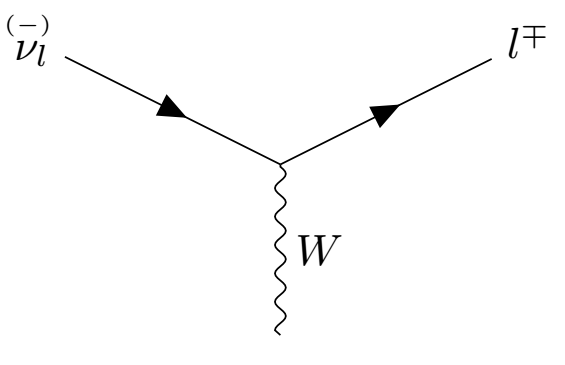
\includegraphics[width=0.4\linewidth]{Plots/Theory/NeutrinoCCInteractionVertices.png}
\hspace{0.1\linewidth}
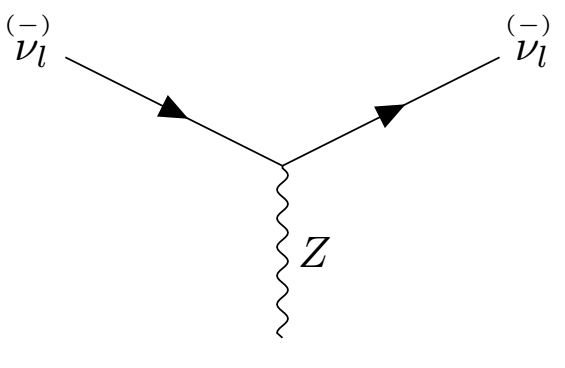
\includegraphics[width=0.4\linewidth]{Plots/Theory/NeutrinoNCInteractionVertices.png}
\caption{Neutrino interaction vertices in the \acrshort{SM}}
\label{fig:FeynmanNuIntVertices}
\end{figure}

%\cite{FundamentalsOfNeutrinoPhysics.pdf} In the SM, the mass of fermions arises as a result of the Higgs mechanism through the presence of Yukawa couplings of the fermion fields with the Higgs doublet. ... a fermion mass term must involve a coupling of left-handed and right-handed fileds, so it is clear that in the SM neutrinos are massless, because their fields do not have a right-handed components

% in weak isospin doublets \cite{FundamentalsOfNeutrinoPhysics.pdf} grouped with their lepton left handed chiral components of charge leptons. Since SM neutrinos do not have a right handed counterpart, they can't acquire mass through the Yukawa lagrangian which combined the left and right handed fields. Their interaction lagrangian is...

%Neutrinos in the \gls{SM} are described as massless with a left-handed chiral field, with no right-handed neutrino chiral field counter part. Neutrinos make a lepton doublet together with their associated leptons. There are no neutrino mass terms in the \gls{SM} Lagrangian and the interaction terms can be divided into two types: the \gls{CC} and the \gls{NC} interactions \cite{FundamentalsOfNeutrinoPhysics.pdf}

%Neutrinos are grouped together with their corresponding charged lepton to form isospin doublets with no right handed neutrino singlet counterpart. In the SM a fermion mass term must involve a coupling of left-handed and right-handed fields and since neutrinos only have left handed fields they can't obtain

%[nuMM/nuElmagInt2015.pdf] However, there was no sign of a neutrino mass. After the discovery of parity violation in 1957, Landau (1957), Lee and Yang (1957), and Salam (1957) proposed the two-component theory of massless neutrinos, in which a neutrino is described by a Weyl spinor and there are only left-handed neutrinos and right-handed antineutrinos. It was, however, clear (Case, 1957; Mclennan, 1957; Radicati and Touschek, 1957) that two-component neutrinos could be massive Majorana fermions and that the two-component theory of a massless neutrino is equivalent to the Majorana theory in the limit of zero neutrino mass. The two-component theory of massless neutrinos was later incorporated in the standard model of Glashow (1961), Weinberg (1967), and Salam (1969), in which neutrinos are massless and have only weak interactions. In the standard model Majorana neutrino masses are forbidden by the $\textsf{SU}\left(2\right)_L\times \textsf{U}\left(1\right)_{\gamma}$ symmetry.

%[nuMM/nuElmagInt2015.pdf] In the standard model of electroweak interactions (Glashow, 1961; Weinberg, 1967; Salam, 1969), neutrinos are described by two-component massless left-handed Weyl spinors (Giunti and Kim, 2007). The masslessness of neutrinos is due to the absence of right-handed neutrino fields, without which it is not possible to have Dirac mass terms, and to the absence of Higgs triplets, without which it is not possible to have Majorana mass terms.

%[OverviewOfNeutrinoPhysicsPheno2024.pdf] three neutrino flavours produced with charged antilepton, or producing a charged lepton in CC weak interaction processes. Therefore neutrino have exhibited a polarisation in a direction that is opposite to their motion, or, equivalently, with negative helicity. For antineutrino it is the opposite. To account for this neutrino are described in the SM with a left handed chiral field $\nu_{\alpha L}\left(x\right)$. In the absence of neutrino masses, this field destroys (creates) neutrinos (antineutrinos) with negative (positive) helicity.  In the SM, neutrinos are considered massless, and no right-handed (RH) neutrino chiral field is included in its content as they would be singlet under the SM gauge group. As such, the corresponding RH neutrinos would be completely inert. Neutrinos and their lepton LH fields form SU(2) doublets $\psi_{\alpha L}\left(x\right)=\left(\nu_{\alpha L}\left(x\right),\alpha_L\left(x\right)\right)$ with hypercharge +1.

%%%%%%%%%%%%%%%%%%%%%%%%%%%%%%%%%%%%%%%%%%%%%%%%%%%%%%%%%%%%%%%%%%%%%%%%%%%%%%%
%%% 2. Neutrino production and sources
The main neutrino sources \cite{FundamentalsOfNeutrinoPhysics.pdf} are the $\beta^-$ decay, which is essentially a neutron decay, happening in radioactive materials, or nuclear reactors, and can be described as
\begin{equation}
n\rightarrow p+e^-+\overline{\nu}_e.
\end{equation}
The source of neutrinos from nuclear reactor was the first artificial source of neutrinos which brought increase of neutrino rate of about $10^7$, as well as higher neutrino energies and enabled the first detection of neutrinos \cite{NeutrinoPhysicsCowanReines.pdf}
Similarly is the $\beta^+$ decay
\begin{equation}
p\rightarrow n+e^++\nu_e
\end{equation}
or the electron capture
\begin{equation}
p+e^-\rightarrow n+\nu_e,
\end{equation}
which occurs in the stars and for Earth especially in the Sun.
Source of $\nu_\mu$ is especially pion, muon and kaon decay, occurring in the atmosphere and the accelerators
\begin{align}
p+X \rightarrow \pi^\pm \rightarrow &\mu^\pm + \nu_\mu\left(\overline{\nu}_\mu\right) \\
 & \mu^\pm \rightarrow e^\pm + \nu_\mu\left(\overline{\nu}_\mu\right) + \nu_e\left(\overline{\nu}_e\right)
\end{align}
Notice that if all muons decay by the time they reach Earth's surface, then there should be almost exactly 2:1 ratio of $\nu_\mu : \nu_e$ for atmospheric neutrinos. This is also used in the modern accelerator based source of neutrinos which have accelerated protons strike a fixed target \cite{GoodmanAdvancesInNeutrinoPhysics.pdf}\cite{SchwartzAccelerators.pdf}.

For supernovas its partly electron capture but 90\% through thermal pair production
\begin{equation}
e^-+e^+\rightarrow\nu_\alpha+\overline{\nu}_\alpha, \alpha=e,\mu,\tau
\end{equation}
There is also cosmic neutrino background that decoupled from the rest of matter shortly after the Big Bang.

%[Master's] The advent of fission reactors brought increase of neutrino rate of about $10^7$, as well as higher neutrino energies, making the neutrino detection worth reinvestigating \cite{NeutrinoPhysicsCowanReines.pdf}. In 1960 Mel Schwartz designed the first neutrino beam made by accelerated protons striking a target, producing pions (mostly), which would decay into neutrinos \cite{GoodmanAdvancesInNeutrinoPhysics.pdf}\cite{SchwartzAccelerators.pdf}.

%%%%%%%%%%%%%%%%%%%%%%%%%%%%%%%%%%%%%%%%%%%%%%%%%%%%%%%%%%%%%%%%%%%%%%%%%%%%%%%
%%% 3. Interaction of neutrinos
Inversely, the detection of neutrinos is usually done by reverting the above mentioned processes.

For example the inverse beta decay
\begin{equation}
\nu +p\rightarrow n+e^+
\end{equation}
was used for the first detection of neutrinos by Cowan and Reines \cite{CowanReinesFirstAttempt.pdf, CowanReinesConfirmation.pdf}. 

%%%%%%%%%%%%%%%%%%%%%%%%%%%%%%%%%%%%%%%%%%%%%%%%%%%%%%%%%%%%%%%%%%%%%%%%%%%%%%%
%%% Masters
%%% Experimental evidence for neutrino %%%
%Soon after Fermi's description of neutrino interaction, in 1934, Bethe and Peierls realized the possibility of reverting the process of beta decay as a mean of direct detection of the neutrino \cite{BethePeierlsDirectDetection.pdf}. For example an interaction in which incident neutrino interacts with proton, transforming it into neutron and creating a positron. From the lifetime of then-known beta decays they estimated the interaction cross-section to be $<\unit[10^{-44}]{cm^2}$ for a neutrino with a few $\unit{MeV}$ energy, or about $10^{-20}$ times the more familiar nuclear values at the time.

%In 1953 C.~L.~Cowan and F.~Reines placed a liquid scintillation detector near the Hanford reactor reporting uncertain results \cite{CowanReinesFirstAttempt.pdf}. They later moved the detector to the Savannah River Plant and in 1956 confirmed \cite{CowanReinesConfirmation.pdf} the detection of the antineutrino, verifying the neutrino hypothesis \cite{NeutrinoPhysicsCowanReines.pdf}.
%(\ovnu{$\nu$} interacting with proton, producing neutron and positron (\ovnu{$\nu$}$+p\rightarrow n+e^+$))

%%% Muon neutrino %%%
Leon Lederman, Jack Steinberger and others joined Schwartz and using a spark chamber detector in 1962 observed\cite{MuonNeutrinoDetection.pdf} a different kind of neutrino, which we now call the muon neutrino ($\nu_{\mu}$), produced in pion decay ($\pi^{\pm}\rightarrow\mu^{\pm} +\nu$), while the previously known neutrino, produced in beta decays, was dubbed the electron neutrino ($\nu_e$).

% Tau neutrino and Z width
In 1990 the L3 Collaboration studied properties of the $Z^0$ boson and fitted to its peak cross-section and decay width to determine the total number of active (interacting with $Z^0$) light ($m_{\nu}<m_{Z}/2$) neutrino flavours ($N_{\nu}$). They found the best fit integer value to be 3 and ruled out the possibility of four or more active light neutrino flavours at $4\sigma$ \cite{ZDecay.pdf}. Latest most precise results put the fitted value to $N_{\nu}=2.9840\pm 0.0082$ \cite{ZDecayPrecise.pdf}.
After this result it was only a matter of time, before the third neutrino, the tau neutrino ($\nu_{\tau}$) was discovered. Evidence for that were shown in 2000 from the DONUT Collaboration at Fermilab \cite{ObservationOfTauNeutrino.pdf}.
%%% End of master's on neutrino history
%%%%%%%%%%%%%%%%%%%%%%%%%%%%%%%%%%%%%%%%%%%%%%%%%%%%%%%%%%%%%%%%%%%%%%%%%%%%%%%

I think I should mention here the basic neutrino interactions and their corresponding cross section. For neutrino on nucleons, the total cross section per neutrino energy is around $\unit[0.7\times 10^{-38}]{cm^2GeV^{-1}}$ for neutrinos and half that for antineutrinos. For neutrino on electron interactions, the total cross section per neutrino energy is more similar to $10^-41-\unit[10^{-42}]{cm^2GeV^{-1}}$.

The main neutrino interactions are
\begin{equation}
\nu_l+n\rightarrow p+l^-
\end{equation}
\begin{equation}
\overline{\nu}_l+p\rightarrow n+l^+
\end{equation}
\begin{equation}
\nu_l+N\rightarrow\nu_l+N
\end{equation}
\begin{equation}
\overline{\nu}_l+N\rightarrow\overline{\nu}_l+N
\end{equation}

\begin{figure}[hbtp]
\centering
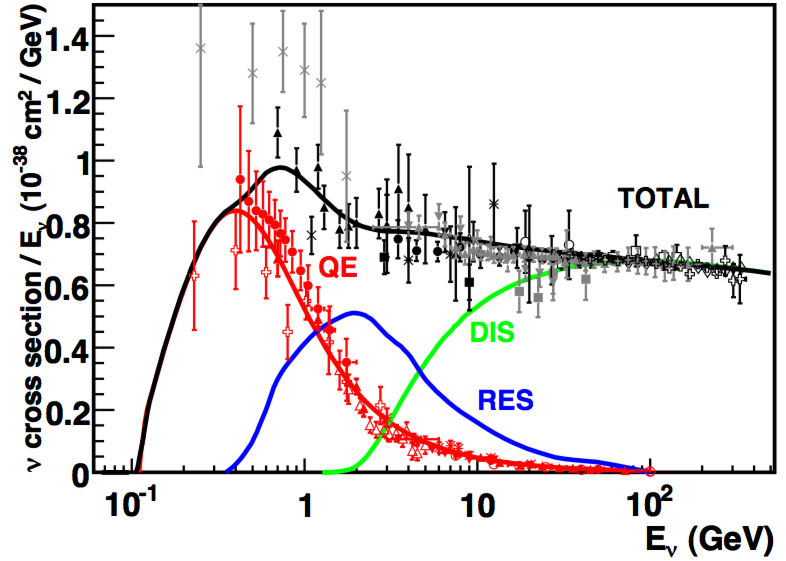
\includegraphics[width=0.8\linewidth]{Plots/Theory/NeutrinoCCCrossSections.png}
\caption{Neutrino \acrshort{CC} cross sections based on the interaction types. Figure from \cite{NeutrinoCCCrossSectionPlot.pdf} compares the measured data \cite{NeutrinoIntOverview2012.pdf} and the prediction \cite{NuanceNuIntSimulation2002.pdf}}
\label{fig:NuCCCrossSection}
\end{figure}


Problems of the SM
%[OverviewOfNeutrinoPhysicsPheno2024.pdf] Besides, the SM falls short in describing other challenging issues, including the long-standing problems of explaining the nature of dark matter [12] and the overabundance of matter over antimatter in the Universe [13]. These fundamental problems may be inter-related, with neutrinos potentially playing a primary role in establishing such connections

\todo{Describe neutrino interactions, CC, NC elastic. QE, Res., DIS. Also nuclear effects - MEC, FSI,...}

\section{Neutrino oscillation}
Neutrino oscillate and therefore have mass. Describe neutrino oscillations and the current status of their measurements. Maybe also when they were discovered and how?

%%%%%%%%%%%%%%%%%%%%%%%%%%%%%%%%%%%%%%%%%%%%%%%%%%%%%%%%%%%%%%%%%%%%%%%%%%%%%%%
%%% Master's on neutrino oscillations
This led B. Pontecorvo, inspired by already known $K^{0}\leftrightarrow \overline{K^0}$ oscillations, to consider $\nu\leftrightarrow\overline{\nu}$ transitions (oscillations), in case the conservation of neutrino charge does not apply\cite{Pontecorvo57.pdf}. Pontecorvo later built upon this statement in 1958 considering that oscillations between $\nu$ and $\overline{\nu}$ are due to them being combinations of particles $\nu_1$ and $\nu_2$ and that the transformation lifetime is related to the mass difference between $\nu_1$ and $\nu_2$ \cite{Pontecorvo58.pdf}, laying foundation for neutrino oscillations as we know them today.

In 1962 Z. Maki, M. Nakagawa and S. Sakata applied Pontecorvo's idea of neutrino oscillations to \textit{weak neutrino} eigenstates $\nu_{\alpha}$ ($\nu_e$, $\nu_{\mu}$) produced in weak interactions. They assumed that oscillation $\nu_{\alpha}\leftrightarrow\nu_{\beta}$ are driven by a non-zero mass difference (therefore if true implying at least one neutrino has a non-zero mass) between \textit{true neutrinos} (= mass neutrino eigenstates $\nu_i$ ($\nu_1$, $\nu_2$)), which are related to weak eigenstates via a linear combination. This relation in general case looks like \cite{MNS1962Osc.pdf}
\begin{equation}
\ket{\nu_{\alpha}}=\sum_{i=1}^{n} U_{\alpha i}^{*}\ket{\nu_{i}},
\end{equation}
where $U$ is a unitary matrix now know as Pontecorvo-Maki-Nakagawa-Sakata (PMNS) matrix and $n$ is the (general) number of light neutrino species \cite{Gonzalez-GarciaNuMassesAndMixing.pdf}.

In the contemporary description of neutrino interactions it is common to treat neutrino as a plane wave  in a relativistic approximation, which after a distance $L$ evolves as \cite{Gonzalez-GarciaNuMassesAndMixing.pdf}
\begin{equation}
\ket{\nu_{\alpha}\left( L\right) }=\sum_{\alpha\sp{\prime}} \sum_{i} U_{\alpha i}^{*} U_{\alpha\sp{\prime} i} e^{-i m_{i}^{2}L/2E} \ket{\nu_{\alpha\sp{\prime}}}.
\end{equation}

Neutrino $\nu_{\alpha}$ can oscillate and therefore be detected as a different neutrino flavour $\nu_{\beta}$ with a probability
\begin{equation}
P_{\nu_{\alpha}\rightarrow\nu_{\beta}}\left( L\right) =\vert\braket{\nu_{\beta}|\nu_{\alpha}\left( L\right) }\vert^{2}=\sum_{i, j}U_{\beta i}U_{\alpha i}^{*}U_{\beta j}^{*}U_{\alpha j}e^{-i\left( m_{i}^{2}-m_{j}^{2}\right) L/2E},
\end{equation}
where the difference of the masses squared is usually denoted as 
\begin{equation}\label{Deltamsq}
\Delta m_{ij}^{2}=m_{i}^{2}-m_{j}^{2}.
\end{equation}

Oscillation probability can be also expressed as
\begin{align}\label{OscProb}
P_{\nu_{\alpha}\rightarrow\nu_{\beta}}\left( L\right)= \delta_{\alpha\beta}
& -4\sum_{i>j}\text{Re} \left( U_{\beta i}U_{\alpha i}^{*} U_{\beta j}^{*}U_{\alpha j}\right)
\sin^{2}\Delta_{ij}\nonumber \\
& +2\sum_{i>j} \text{Im} \left( U_{\beta i}U_{\alpha i}^{*}U_{\beta j}^{*}U_{\alpha j}\right) \sin 2\Delta_{ij},
\end{align}
where\cite{Gonzalez-GarciaNuMassesAndMixing.pdf} \[\Delta_{ij}\equiv\Delta m_{ij}^{2}\frac{L}{4E}=1.267\frac{\Delta m_{ij}^{2}}{\unit{eV^2}}\frac{L/E}{\unit{m}/\unit{MeV}} .\]

Since real neutrino beams are not monochromatic, what is measured in experiments is an \textbf{average} oscillation probability with $\left\langle \sin^{2}\Delta_{ij}\right\rangle$ and $\left\langle\sin2\Delta_{ij}\right\rangle $ in eq.\ref{OscProb}. We can notice that if $E/L\gg\Delta m_{ij}^{2}$ the oscillation does not show any effect yet and if $E/L\ll\Delta m_{ij}^2$ the oscillating phase goes through many cycles and is averaged to $\left\langle \sin^{2}\Delta_{ij}\right\rangle=1/2$. Therefore different experimental settings can measure different oscillation parameters \cite{PDG.pdf}.

Several experimental indications for neutrino oscillations were found shortly after its theoretical predictions.
Davis continued looking for $^{37}Ar$ in a detector with $^{37}Cl$, but now moving to Homestake Gold Mine with Harmer and Hoffman focusing on detecting the first electron neutrinos from the Sun \cite{Homestake1998.pdf}. Already in 1968 their Homestake Solar Neutrino Observatory saw a solar neutrino flux less than 3 Solar Neutrino Units (SNU = one interaction per $10^{36}$ target atoms $\unit{s^{-1}}$), well below the solar model prediction of the time \cite{Homestake1968.pdf}. This discrepancy became the \textit{“solar neutrino problem”}, which is in line with neutrino oscillations, but no direct implications could have been drawn since it might have been caused by a lack of understanding of nuclear physics, astrophysics of the Sun, or particle physics of the neutrino\cite{GoodmanAdvancesInNeutrinoPhysics.pdf}.

In 2002, Raymond Davis was together with Masatoshi Koshiba awarded the Nobel prize "for pioneering contributions to astrophysics, in particular for the detection of cosmic neutrinos" \cite{Nobel}. Koshiba was part of the Kamiokande experiment, which confirmed the results from Homestake \cite{Kamiokande96.pdf}.

Possible explanation of the Solar neutrino problem was proposed in 1978 by L. Wolfenstein, who considered the effect of matter on neutrino oscillations \cite{Wolfenstein78.pdf}. His modification of neutrino oscillations when passing through matter arises from the coherent forward scattering of electron neutrinos, as a result of their charged current (CC) interaction with electrons, which are abundant in matter, as opposed to other lepton flavours, muons and tauons, resulting in an imbalance between $\nu_e$ and $\nu_{\mu}/\nu_{\tau}$. This manifests as an effective potential, which depends on the density and composition of the matter \cite{Wolfenstein78.pdf}. This idea was later further developed for neutrinos passing through the Sun by Mikheyev and Smirnov in 1985 \cite{MikheyevSmirnov85.pdf}\cite{Gonzalez-GarciaNuMassesAndMixing.pdf} and we now call this effect the Mikheyev-Smirnov-Wolfenstein (MSW) effect.

To showcase this effect we consider only two neutrino flavours, $\nu_e$ and $\nu_X$, where $X$ denotes a combination of all other non-electron flavours. Vacuum oscillations are in this two-neutrino approximation driven by a single mass splitting $\Delta m^2$ and the corresponding PMNS matrix is a rotational matrix parametrized by one angle $\theta$:
\begin{equation}
U=
\begin{pmatrix}
 \cos\theta  & \sin\theta    \\
 -\sin\theta & \cos\theta
\end{pmatrix}.
\end{equation}

The MSW effect can be described as the presence of an Effective Potential \cite{CERNSchool2001.pdf}
\begin{equation}
V=\pm\sqrt{2}G_{F}N_{e}=\pm 3.8\times 10^{-14}\left(\frac{\rho}{\unit{g}\ \unit{cm^{-3}}}\right)\left(\frac{Y_e}{0.5}\right)\unit{eV},
\end{equation}
where $G_F$ is the Fermi coupling constant, $N_e$ is the electron density, $Y_e$ is the electron number per nucleon and plus or minus sign is for neutrinos or antineutrinos respectively.

This potential can be seen as having the effect of modifying the $\Delta m^2$ and $\theta$ of the neutrino oscillations: \cite{CERNSchool2001.pdf}
\begin{equation}\label{MSWEffect}
\sin^22\theta_m=\frac{\sin^22\theta}{\sin^22\theta+\left(\cos 2\theta\mp\xi\right)^2}
\end{equation}
\begin{equation}
\left(\Delta m^2\right)_{\textsl{eff}}=\Delta m^2\times\sqrt{\sin^22\Theta+\left(\cos 2\theta\mp\xi\right)^2},
\end{equation}
where 
\begin{equation}
\xi=\frac{2\sqrt{2}G_FN_e}{\Delta m^2}.
\end{equation}

%Atmospheric neutrino experiments - atmospheric neutrino anomaly - how many neutrinos
Measuring atmospheric neutrinos brought about another neutrino conundrum, the \textit{Atmospheric neutrino anomaly}. It came from the disagreement between experiments such as NUSEX\cite{NUSEX89.pdf} and Fr\'{e}jus\cite{Frejus95.pdf}, which used iron calorimeters detectors, and experiments IMP\cite{IMP92.pdf} and Kamiokande\cite{Kamiokande94.pdf}, which used water Cherenkov detectors. All of these experiments were looking for a deficit of $\nu_{\mu}$, or an excess of $\nu_e$, compared to prediction. While the first two experiments saw a good agreement between experimental results and predictions, the latter two did not and suggested the possibility of neutrino oscillations, which could explain their disagreement. 

Solution to the Atmospheric neutrino anomaly came in 1998, when the Super-Kamiokande (SK) experiment showed for the first time the~experimental evidence for neutrino oscillations \cite{EvidenceForAtmoOscFirstEverOscRes.pdf}. SK has however also disfavoured the two neutrino hypothesis, with regards to the existence of an additional neutrino flavour. 

The Solar neutrino anomaly was also resolved, when the Sudbury Neutrino Observatory (SNO) provided $>5\sigma$ evidence for  solar $\nu_e$ oscillations in 2002, independent on the solar model \cite{NCOscInSNOSecondOscResult.pdf}. While other solar neutrino experiments measured solar $\nu_e$ only via the charged current (CC) interactions
\begin{equation}
\nu_e+n\rightarrow p+e^- \qquad (CC),
\end{equation}
SNO had an ability to also detect neutrinos via the neutral current (NC) interaction
\begin{equation}
\nu+X\rightarrow\nu+X^{\prime} \qquad (NC),
\end{equation}
which are equally sensitive to all active neutrino flavours and their rate is therefore unaffected by standard neutrino oscillations. SNO could compare CC and NC event rates and conclude that $\nu_e$ from the Sun oscillate into other neutrino flavours along the way \cite{NCOscInSNOSecondOscResult.pdf}.

Takaaki Kajita from SK and Arthur B. McDonald from SNO were jointly awarded the Nobel Prize in 2015 "for the discovery of neutrino oscillations, which shows that neutrinos have mass" \cite{Nobel}.

In 1990 the L3 Collaboration studied properties of the $Z^0$ boson and fitted to its peak cross-section and decay width to determine the total number of active (interacting with $Z^0$) light ($m_{\nu}<m_{Z}/2$) neutrino flavours ($N_{\nu}$). They found the best fit integer value to be 3 and ruled out the possibility of four or more active light neutrino flavours at $4\sigma$ \cite{ZDecay.pdf}. Latest most precise results put the fitted value to $N_{\nu}=2.9840\pm 0.0082$ \cite{ZDecayPrecise.pdf}.
After this result it was only a matter of time, before the third neutrino, the tau neutrino ($\nu_{\tau}$) was discovered. Evidence for that were shown in 2000 from the DONUT Collaboration at Fermilab \cite{ObservationOfTauNeutrino.pdf}.

The PMNS matrix describing neutrino oscillations in the so~called $3\nu$ para-digm depends on six independent parameters: 3 mixing angles ($\theta_{12}$, $\theta_{13}, \theta_{23}$) and 3 phases. One of the phases is $\delta_{CP}$, which, if different from 0 or $\pi$, implies CP violation, and the other two are $\alpha$ and $\beta$, so called Majorana phases, which are non zero only if neutrinos are Majorana (neutrinos and antineutrinos are described by just one field, i.e. neutrinos are the same particle as antineutrinos). Majorana phases play no role in neutrino oscillations, so they are usually left out in the description \cite{PDG.pdf}. The PMNS matrix in this case can be parametrized as

\[
U=
\begin{pmatrix}
 U_{e1}     & U_{e2}     & U_{e3}    \\
 U_{\mu 1}  & U_{\mu 2}  & U_{\mu 3} \\
 U_{\tau 1} & U_{\tau 2} & U_{\tau 3}
\end{pmatrix}
=
\]
\begin{equation}\label{param3}
=
\begin{pmatrix}
 1 & 0       & 0      \\
 0 & c_{23}  & s_{23} \\
 0 & -s_{23} & c_{23}
\end{pmatrix}
\begin{pmatrix}
 c_{13}              & 0 & s_{13}e^{-i\delta} \\
 0                   & 1 & 0                  \\
 -s_{13}e^{i\delta} & 0 & c_{13}
\end{pmatrix}
\begin{pmatrix}
 c_{12}  & s_{12} & 0 \\
 -s_{12} & c_{12} & 0 \\
 0       & 0      & 1
\end{pmatrix}
\begin{pmatrix}
 1 & 0           & 0 \\
 0 & e^{i\alpha} & 0 \\
 0 & 0           & e^{i\beta}
\end{pmatrix},
\end{equation}
where $c_{ij}\equiv\cos\theta_{ij}$ and $s_{ij}\equiv\sin\theta_{ij}$.

Other than the PMNS matrix, neutrino oscillations depend on the mass squared differences (eq.\ref{Deltamsq}). In case of 3 neutrinos, those are $\Delta m^2_{21}$ and $\Delta m^2_{31}$. $\Delta m^2_{21}$ mainly drives oscillations of solar neutrinos and is therefore often denoted as $\Delta m^2_{\odot}$ or $\Delta m^2_{sol}$, while $\Delta m^2_{31}$ drives oscillations on the scale for atmospheric neutrinos  and is often written as $\Delta m^2_{atm}$ \cite{Gonzalez-GarciaNuMassesAndMixing.pdf}. There can only be two independent mass squared differences for oscillation of three neutrinos, since 
\begin{equation}
\Delta m^2_{21} + \Delta m^2_{32} + \Delta m^2_{13} = 0.
\end{equation}
%%% End of master's on neutrino oscillations
%%%%%%%%%%%%%%%%%%%%%%%%%%%%%%%%%%%%%%%%%%%%%%%%%%%%%%%%%%%%%%%%%%%%%%%%%%%%%%%

\section{Neutrino masses}
Experiments for their values? Theoretical predictions for how they obtained them

Theories of neutrino mass generation

[Fundamentals of neutrinos physics and astrophysics]
The only extension of the SM that is needed is the introduction of right-handed components $\nu_{\alpha R}$ of the neutrino fields. Such a model is sometimes called the \textit{minimally extended Standard Model}. The right handed neutrino fields are fundamentally different from the other elementary fermion fields because they are invariant under the symmetries of the SM: they are \textbf{singlets} of $\textsf{SU}(3)_C\times\textsf{SU}(2)_L$ and have hypercharge $Y=0$. The right handed neutrino fields are called sterile [883] because they do not participate in weak interactions and their only interaction is gravitational. their right handedness is not required though! could also be left handed but have to be singlets and therefore sterile!

In the minimally extended standard model with three right handed neutrino fields, the SM Higgs-lepton Yukawa Lagrangian is extended by adding a lepton term with the same structure as the second term on the right handed side, which generates the masses of up-type quarks
\begin{equation}
\mathcal{L}_Y=
-\sum_{\alpha,\beta=e,\mu,\tau} Y_{\alpha\beta}^{\prime l} \overline{L}_{\alpha L}\Phi l_{\beta R}^{\prime}
-\sum_{\alpha,\beta=e,\mu,\tau} Y_{\alpha\beta}^{\prime \nu} \overline{L}_{\alpha L}\tilde{\Phi} \nu_{\beta R}^{\prime}
+\textsf{h.c.},
\end{equation}
where $Y^{\prime \nu}$ is a new matrix of Yukawa couplings.

Using the unitary gauge we can diagonalize the Yukawa couplings we obtain
\begin{equation}
\mathcal{L}_Y=
-\sum_{\alpha=e,\mu,\tau}\frac{y_\alpha^l v}{\sqrt{2}}\overline{l}_\alpha l_\alpha
-\sum_{k=1}^N \frac{y_k^\nu v}{\sqrt{2}}\overline{\nu}_k\nu_k
-\sum_{\alpha=e,\mu,\tau}\frac{y_\alpha^l}{\sqrt{2}}\overline{l}_\alpha l_\alpha H
-\sum_{k=1}^N \frac{y_k^\nu}{\sqrt{2}}\overline{\nu}_k\nu_k H
\end{equation}

Therefore the neutrino masses are given by
\begin{equation}
m_k=\frac{y_k^\nu v}{\sqrt{2}}\,\,\,\left(k=1,...,N\right),
\end{equation}
and massive Dirac neutrinos couple to the Higgs field through the last term. Note that the neutrinos masses are proportional to the Higgs VEV $v$, as the masses of charged leptons and quarks. However, it is known that the masses of neutrinos are much smaller than those of charged leptons and quarks, but there is no explanations here of the very small values of the eigenvalues $Y_k^{\nu}$ of the Higgs-neutrino Yukawa coupling matrix that are needed. The lagrangian defined this way does not conserve the lepton flavour number, which leads to neutrino oscillations. The Dirac character of massive neutrinos is closely related to the invariance of the total Lagrangian under the global U(1) gauge transformations.

The sterile neutrino fields do not participate in weak interaction with both their left and right components, but can couple with the ordinary neutrinos through the mass therm, generating a complicated mixing between active and sterile degrees of freedom.Since at present there is no indication of the existence of such additional sterile Dirac neutrino fields, ockham's razor suggests to ignore them...

%[nuMM/nuElmagInt2015.pdf] We now know that neutrinos are massive, because many experiments observed neutrino oscillations (Giunti and Kim, 2007; Bilenky, 2010; Xing and Zhou, 2011; Beringer et al., 2012; Gonzalez-Garcia et al., 2012; Bellini et al., 2014), which are generated by neutrino masses and mixing (Pontecorvo, 1957, 1958, 1968; Maki, Nakagawa, and Sakata, 1962). Therefore, the standard model must be extended to account for the neutrino masses. There are many possible extensions of the standard model that predict different properties for neutrinos (Ramond, 1999; Mohapatra and Pal, 2004; Xing and Zhou, 2011). Among them, most important is their fundamental Dirac or Majorana character. In many extensions of the standard model neutrinos also acquire electromagnetic properties through quantum loop effects which allow direct interactions of neutrinos with electromagnetic fields and electromagnetic interactions of neutrinos with charged particles.

\subsection{Majorana neutrinos}
[Fundamentals of neutrinos physics and astrophysics,p.190]
If the neutrino is massless, since the left handed chiral component of the neutrino field obeys the Weyl equation in both the Dirac and Majorana descriptions and the right handed chiral component is irrelevant for neutrino interactions, the Dirac and Majorana theories are physically equivalent. From this it is clear that in practice one can distinguish a Dirac from a Majorana neutrino only by measuring some effect due to the neutrino mass. Moreover, the mass effect must not be of kinematical nature, because the kinematical effects of Dirac and Majorana masses are the same. For example, the Dirac and Majorana nature of neutrinos cannot be revealed through neutrino oscillations! The most promising way to find if neutrinos are Majorana particles is the search for neutrinoless double beta decay.

[OverviewOfNeutrinoPhysicsPheno2024.pdf] In contrast, the Majorana phases do not enter the flavour neutrino oscillation probabilities [22, 85], but contribute to the $\beta\beta_{0\nu}$ decay rate